\section{Backend-Logik}\label{Sec:Backend-Logik}

Die Logik des Feasibility-Check-Algorithmus besteht aus vier zentralen Methoden, die zusammen die Prüfung der Machbarkeit eines Tests realisieren. Zum einen gibt es eine Helfer-Methode, die den eigentlichen Algorithmus aufruft und sicherstellt, dass der Aufrufer der REST-API eine aussagekräftige Rückmeldung erhält. Die Kernkomponente bildet die \texttt{FeasibilityCheck()}-Methode, welche abhängig von der Art der Überprüfung den Condition oder den Equipment Check aufruft. Beide Prüfungen sind als eigenständige Methoden implementiert. Der gesamte Ablauf wird durch vier Aktivitäts- bzw. Flussdiagramme visualisiert. In diesen Diagrammen werden Schleifen durch farblich hervorgehobene Bereiche dargestellt, die jeweils einen gleichfarbigen Kreis als Einstiegspunkt sowie einen zweiten als Ausstiegspunkt enthalten.

Die Ausführung des Algorithmus wird initiiert, sobald der Benutzer im Frontend einen \textit{Button} in der Weboberfläche betätigt. Dies löst einen asynchronen HTTP-Call über eine REST-API aus, welcher die Helfer-Methode \texttt{CheckFeasibility()} aufruft und die Test-ID des zu überprüfenden Tests als Argument übergibt.

\begin{figure}[!htbp]
    \centering
    \makebox[\textwidth]{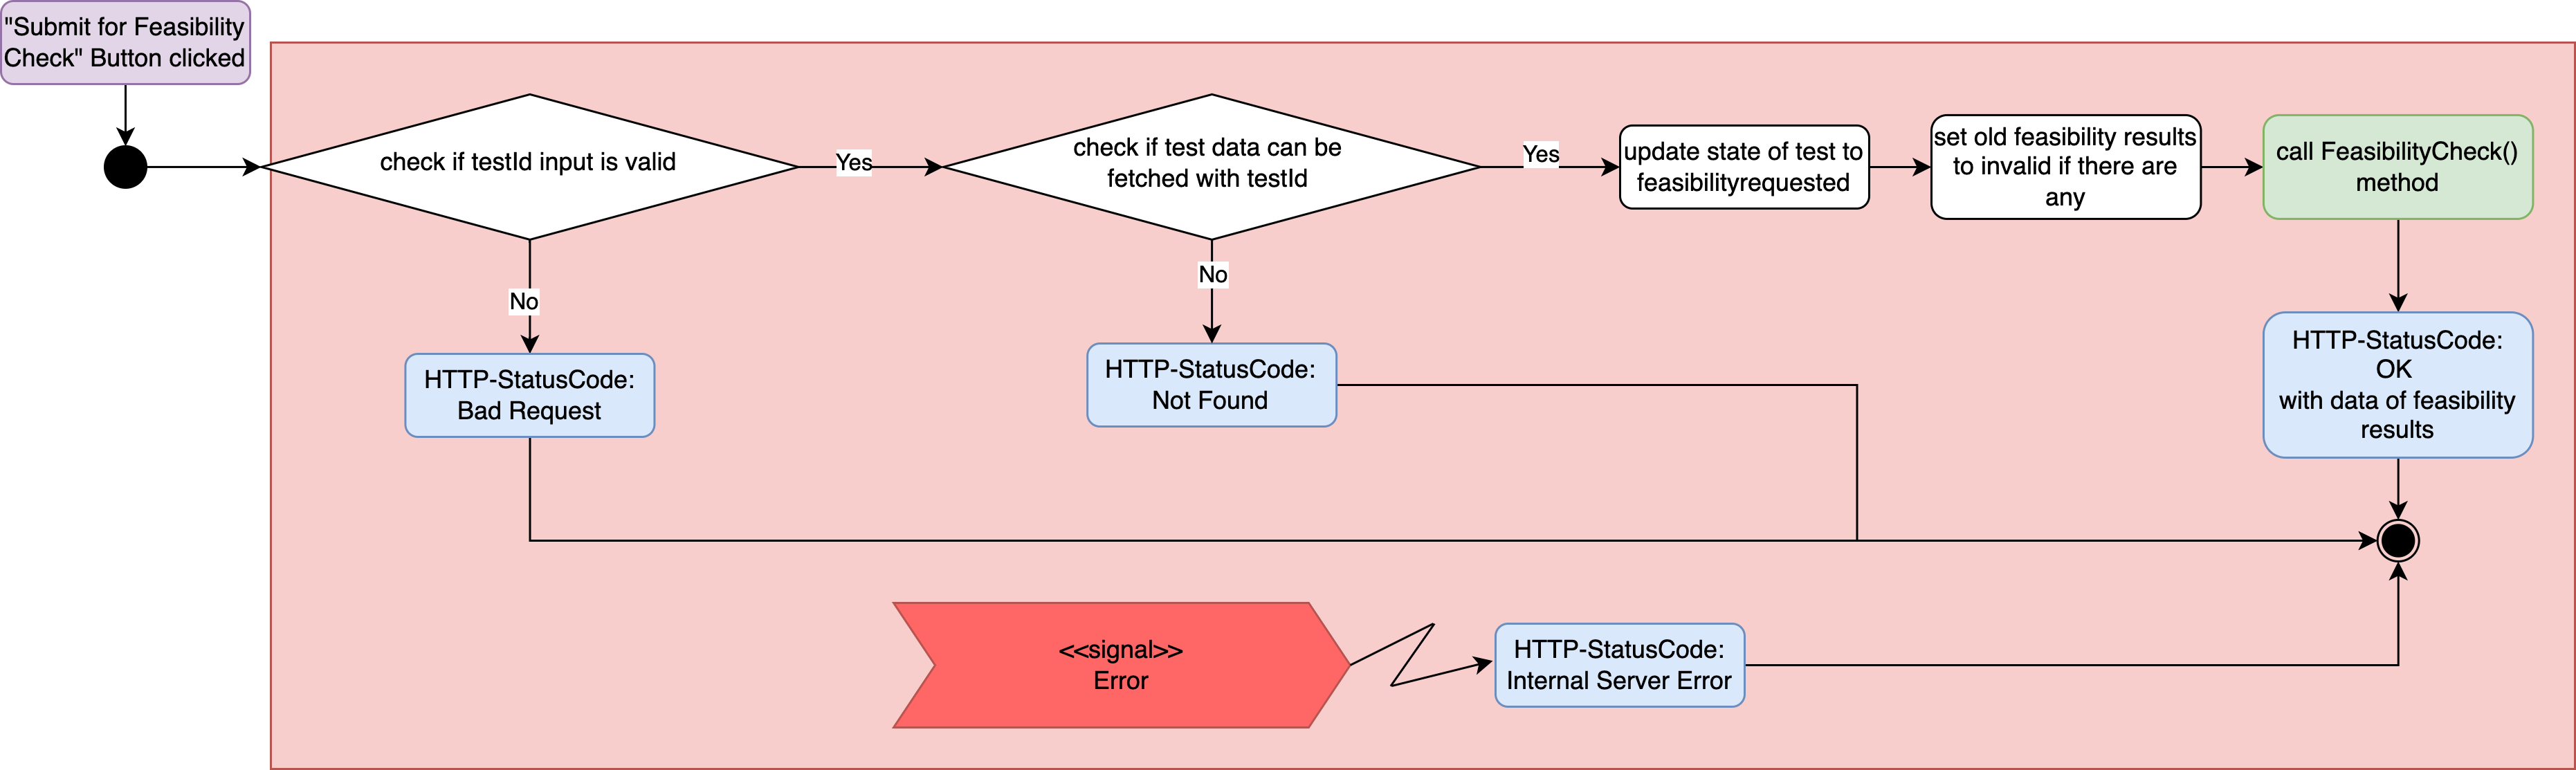
\includegraphics[width=0.85\paperwidth]{bilder/flowchart-check-feasibility-http-call-6-2.png}}
    \caption{Flussdiagramm der Helfer-Methode \texttt{CheckFeasibility()}}
    \label{fig:feasibility-http-call-method}
\end{figure}

Der Ablauf dieser Helfer-Methode ist in Abbildung \ref{fig:feasibility-http-call-method} dargestellt. Ihre Hauptaufgabe besteht darin, die eigentliche \texttt{FeasibilityCheck()}-Methode (grünes Rechteck in der Graphik \ref{fig:feasibility-http-call-method}) auszuführen und zusätzlich eine geeignete HTTP-Statusmeldung an das Frontend bzw. den Benutzer zurückzugeben. Zusätzlich wird vor der Verarbeitung die übergebene Test-ID auf Gültigkeit überprüft und der Test-Status auf \texttt{FEASIBILITYREQUESTED} aktualisiert. Falls der FeasibilityCheck für diesen Test bereits zuvor durchgeführt wurde, müssen alte Ergebnisse in der Datenbank noch als ''invalid'' markiert.


Zur besseren Übersicht wird in Abbildung \ref{fig:feasibility-http-call-method} auch der initiale Button-Klick im Frontend als Aktivität (lila markiert) dargestellt. Die eigentliche Logik beginnt jedoch erst nach dem schwarzen Einstiegspunkt, der den Start des Algorithmus kennzeichnet.

\begin{figure}[!htbp]
    \centering
    \makebox[\textwidth]{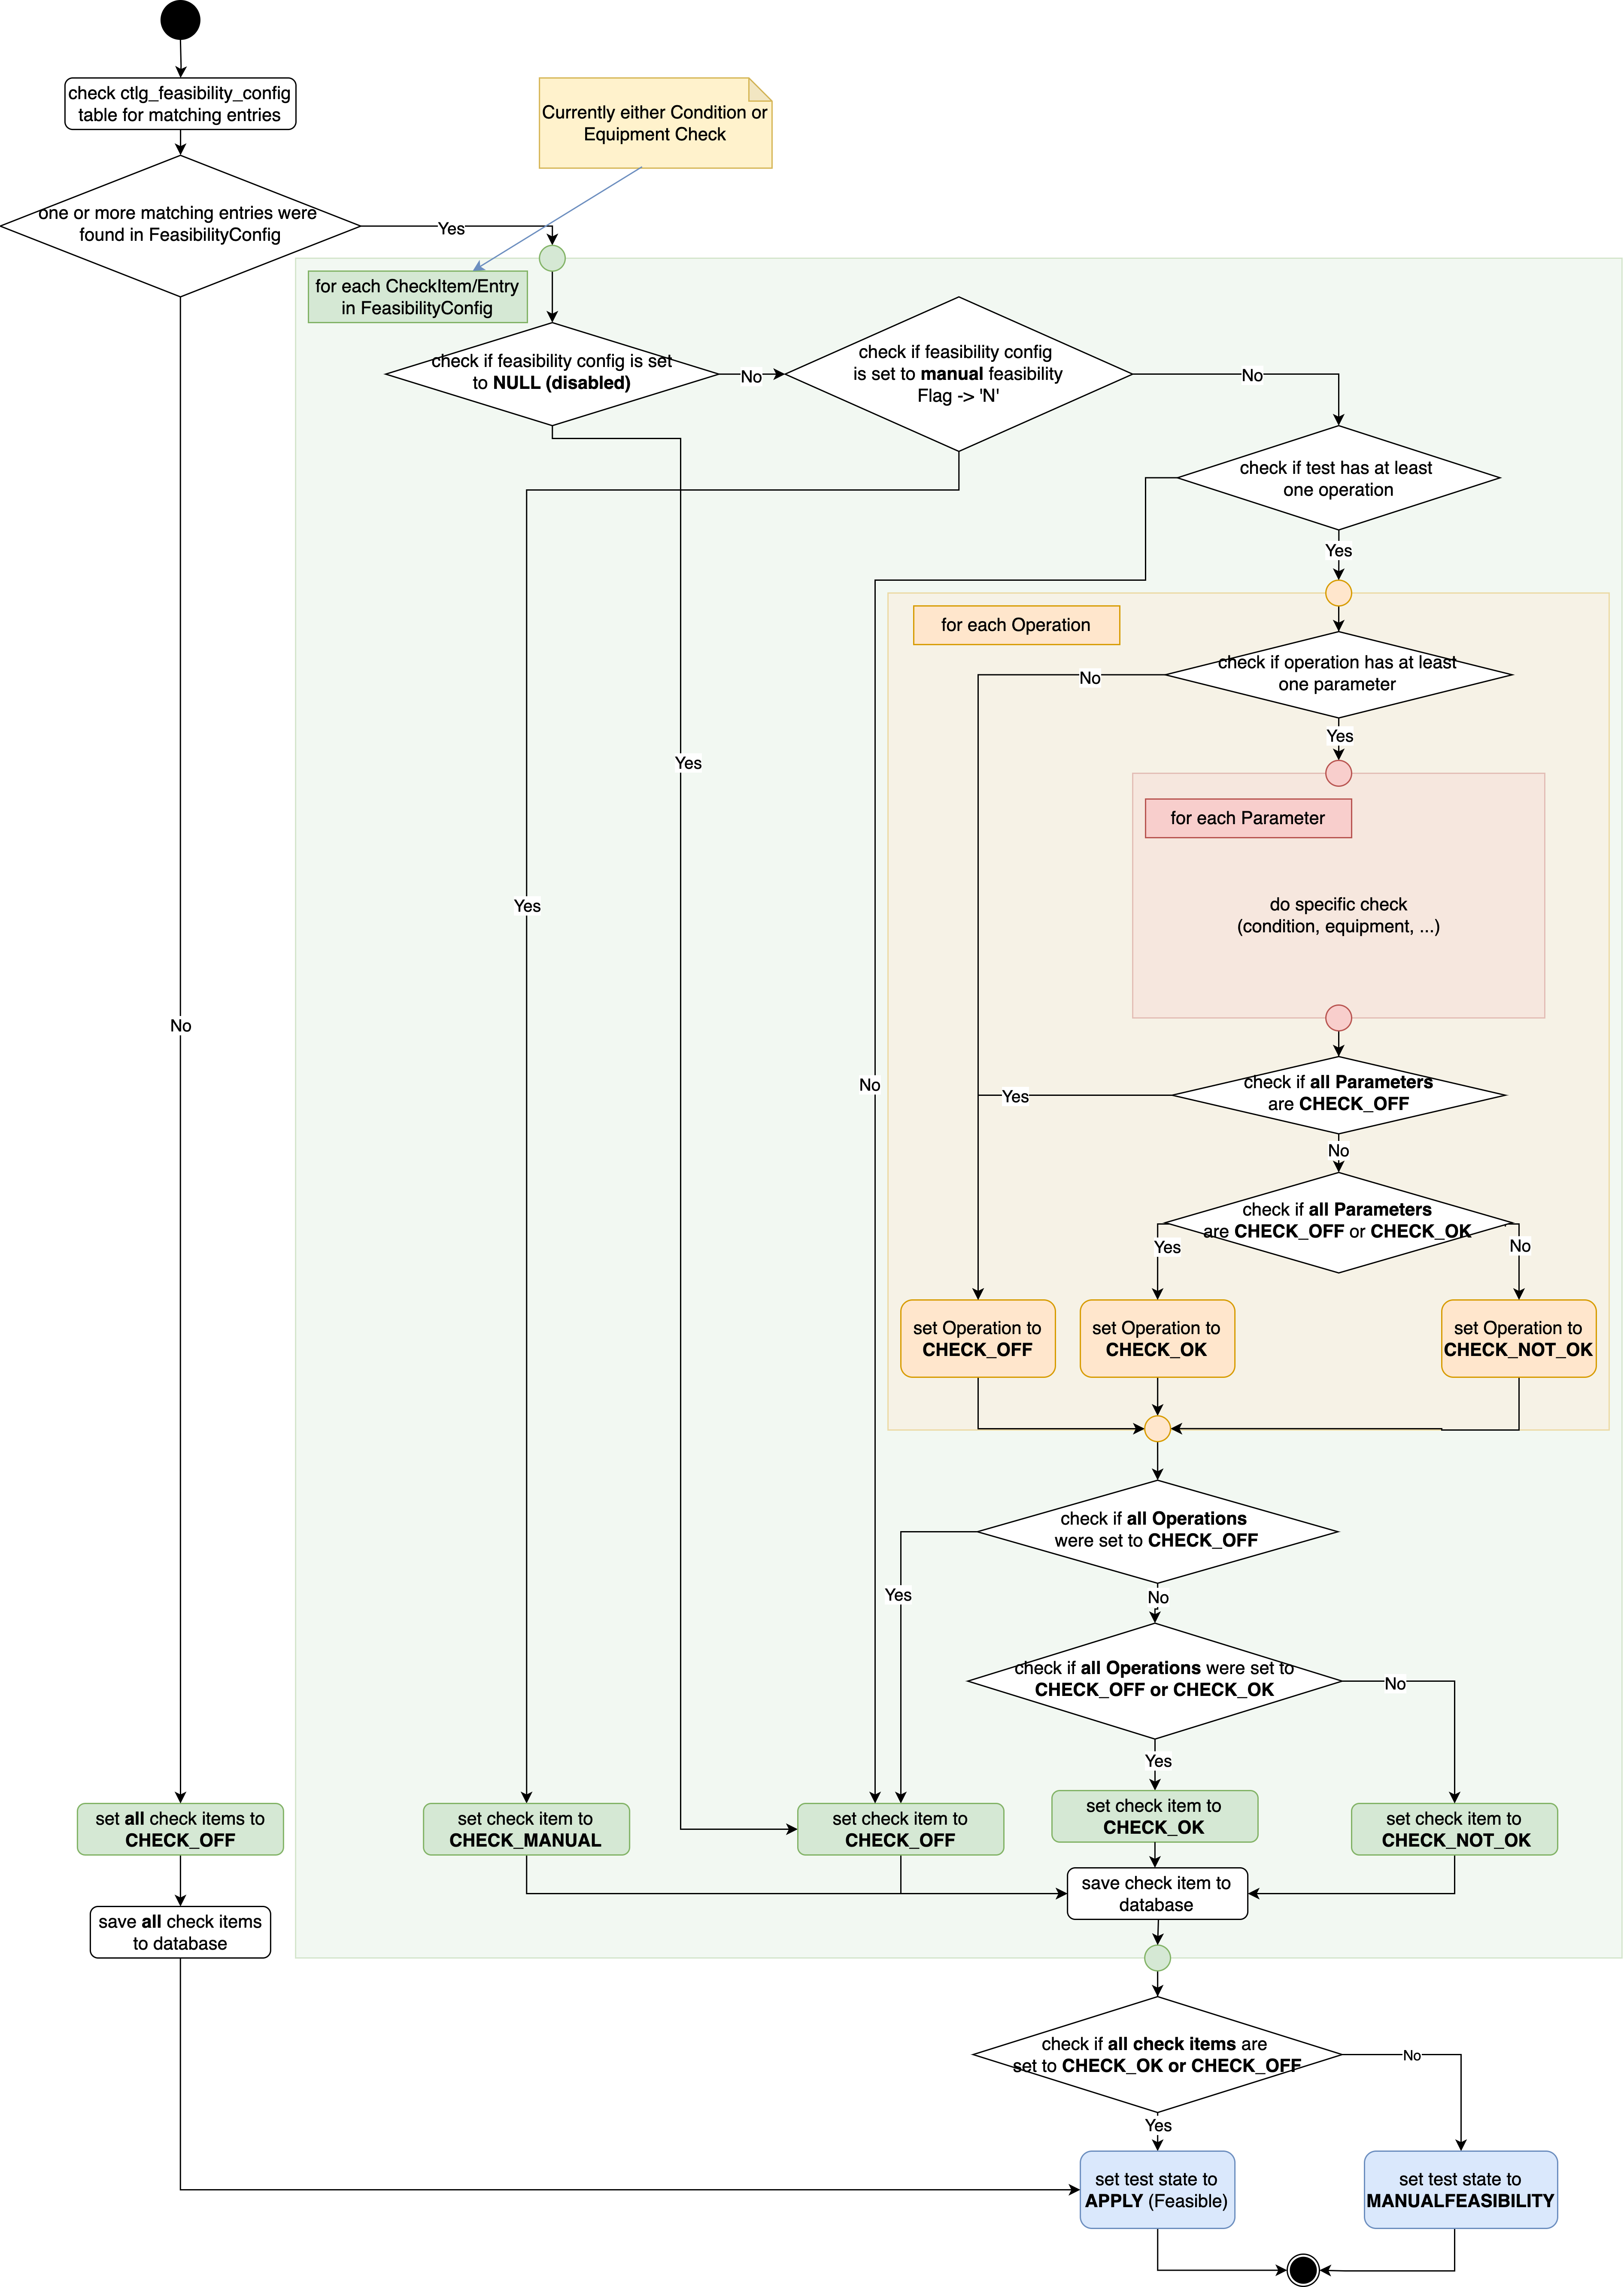
\includegraphics[width=0.85\paperwidth]{bilder/flowchart-feasibilitycheck-modiefied-for-thesis-6-2.png}}
    \caption{Flussdiagramm des Feasibility Check}
    \label{fig:feasibility-check}
\end{figure}

Die Kernlogik des Feasibility Checks wird durch die Methode \texttt{FeasibilityCheck()} ausgeführt, die im Flussdiagramm in Abbildung \ref{fig:feasibility-check} detailliert dargestellt ist. Diese Methode erhält von der Helfer-Methode die Test-ID und überprüft die \textit{Feasibility} des Tests anhand der relevanten Parameter und Operationen. Um die Logik des Algorithmus zu vereinfachen, wird ein Enum eingeführt, das den Status einzelner \textit{Teil-Checks} kennzeichnet. Dieser besteht aus vier möglichen Stati mit jeweils spezifischer Bedeutung:

\begin{table}[htbp]
    \centering
    \footnotesize
    \renewcommand{\arraystretch}{1.3} % Erhöht den Zeilenabstand
    \begin{tabular}{p{0.25\linewidth} p{0.7\linewidth}}
        \toprule
        \textbf{Status} & \textbf{Beschreibung} \\
        \midrule
        \texttt{CHECK\_OFF} & Der Check ist deaktiviert; eine Überprüfung ist weder erforderlich noch vorgesehen. Dies ist insbesondere der Fall, wenn ein Parameter bzw. eine Operation keine Stressoperation darstellt und somit keine PlanValue definiert werden muss. \\
        \midrule
        \texttt{CHECK\_OK} & Der Check war erfolgreich. \\
        \midrule
        \texttt{CHECK\_NOT\_OK} & Der Check war nicht erfolgreich oder es ist ein Fehler aufgetreten. \\
        \midrule
        \texttt{CHECK\_MANUAL} & Eine automatische Überprüfung ist nicht möglich oder der Check ist noch nicht für die automatisierte Überprüfung zugelassen; der Check muss von einem Mitarbeiter manuell durchgeführt werden. \\
        \bottomrule
    \end{tabular}
    \caption{Stati von Feasibility-Teil-Checks, gespeichert als \texttt{FCIR\_STATE} in Feasibility Result (\texttt{feasibility\_check\_item\_result}))}
    \label{tab:feasibility-states}
\end{table}

Jede zu überprüfende Einheit – sei es auf der Ebene des Parameters, der Operation oder des CheckItems – erhält einen entsprechenden Status. Der Algorithmus arbeitet hierarchisch: Zunächst erfolgt die Bewertung auf der untersten Ebene, also bei den Parametern, sofern diese vorhanden sind. Enthält ein Test Operationen, so werden diese Operationen und deren Parameter einzeln bewertet. Für jeden Parameter, der ein prüfbares Ergebnis liefert, wird ein Feasibility-Ergebnis in der Datenbank gespeichert. Enthält ein Test zwar Operationen, diese jedoch keine Parameter, erfolgt die Speicherung ausschließlich auf der Ebene der Operation. Besitzt ein Test gar keine Operationen (und somit auch keine Parameter), wird lediglich ein Gesamtergebnis für den Test abgelegt.

Obwohl die Ergebnisse der untergeordneten Ebenen zu einem Gesamtstatus aggregiert werden – beispielsweise durch die Zusammenfassung der Parameterwerte zu einem Operationsergebnis (siehe orange markierte Aktivitäten in Abb. \ref{fig:feasibility-check}) und der Operationsergebnisse zu einem CheckItem-Ergebnis (sei es ein \gls{ConditionCheck} oder \gls{EquipmentCheck}, dargestellt in den grünen Aktionen) – wird in der Datenbank ausschließlich das Ergebnis der jeweils untersten vorhandenen Ebene persistent abgelegt. Durch diese Maßnahme in Kombination mit der bewussten Nicht-Speicherung von Ergebnissen, die lediglich den Status \texttt{CHECK\_OFF} aufweisen, wird eine unnötige Datenbankaufblähung vermieden und die Systembelastung reduziert, da diese Ergebnisse keine zusätzlichen, benutzerrelevanten Informationen liefern. Zudem wird der Persistierungsvorgang in den Flussdiagrammen nicht explizit dargestellt, da die Speicherung auf unterschiedlichen Ebenen erfolgen und eine detaillierte Visualisierung die Diagramme erheblich komplizierter machen würde.

Basierend auf den Ergebnissen aller CheckItems wird schließlich der finale Test-Status bestimmt. Dieser kann entweder den Wert \textbf{''APPLY''} (''FEASIBLE''; erfolgreich) oder \textbf{''MANUALFEASIBILITY''} (manuelle Prüfung erforderlich) (blau markierte Aktivitäten) annehmen.

Um es zu ermöglichen, dass bestimmte \textit{CheckItems} für einen Test in der Konfiguration vollständig deaktiviert werden können – wobei dies im System als erfolgreiche Überprüfung gewertet wird – kann das entsprechende Flag in der Feasibility-Konfiguration entweder leer (\textit{null}) gelassen werden oder es wird für das betreffende CheckItem gar kein Eintrag in der Konfigurations-Tabelle erstellt. \todo{Beispiel}

\textbf{Konkreter Ablauf des Feasibility Check Algorithmus} \\
Zunächst werden die für den Test hinterlegten Konfigurationen für jedes \texttt{CheckItem} aus der Datenbank abgerufen. Falls kein Eintrag existiert, wird der Check automatisch als erfolgreich gewertet. Ist das zugehörige Flag auf 'N' gesetzt, muss die Überprüfung manuell erfolgen, und der Check ist an dieser Stelle beendet. Nur wenn das Flag auf 'Y' gesetzt ist, wird das entsprechende \textit{CheckItem} (Condition oder \gls{EquipmentCheck}) tatsächlich geprüft.

Anschließend wird überprüft, ob der Test mindestens eine Operation enthält. Falls ja, wird jede dieser Operationen durchlaufen, um festzustellen, ob sie einen oder mehrere Parameter besitzt. Für jeden Parameter wird dann – abhängig vom \textit{CheckItem} – entweder der \gls{ConditionCheck} oder der \gls{EquipmentCheck} durchgeführt.

\subsection{Condition Check}



Der Ablauf des \gls{ConditionCheck} ist in Abbildung \ref{fig:condition-check} dargestellt. Zunächst wird die relevante Verknüpfungstabelle \texttt{op\_data\_param\_type} aus der Datenbank abgerufen. Diese Tabelle definiert den zulässigen Wertebereich eines Parameters durch einen minimalen und maximalen Wert. Falls weder ein minimaler noch ein maximaler Wert definiert ist, wird der \textit{Parameter-Teil-Check} auf \texttt{CHECK\_OFF} gesetzt, was bedeutet, dass keine Überprüfung erforderlich ist und der Parameter automatisch als gültig betrachtet wird. Sind sowohl ein minimaler als auch ein maximaler Wert hinterlegt, muss zusätzlich ein geplanter Wert (\textit{PlanValue}) für den Parameter vorhanden sein. Liegt dieser innerhalb des zulässigen Bereichs, gilt die Sinnhaftigkeitsprüfung als erfolgreich, und der nächste Parameter der Operation wird verarbeitet. 

In Sonderfällen, in denen lediglich ein Mindest- oder Höchstwert vorliegt, genügt es, wenn der PlanValue die entsprechende Bedingung (über dem Mindestwert oder unter dem Höchstwert) erfüllt – diese Fälle sind im Flussdiagramm zur besseren Übersichtlichkeit nicht dargestellt.

\begin{figure}[!htb]
    \centering
    \makebox[\textwidth]{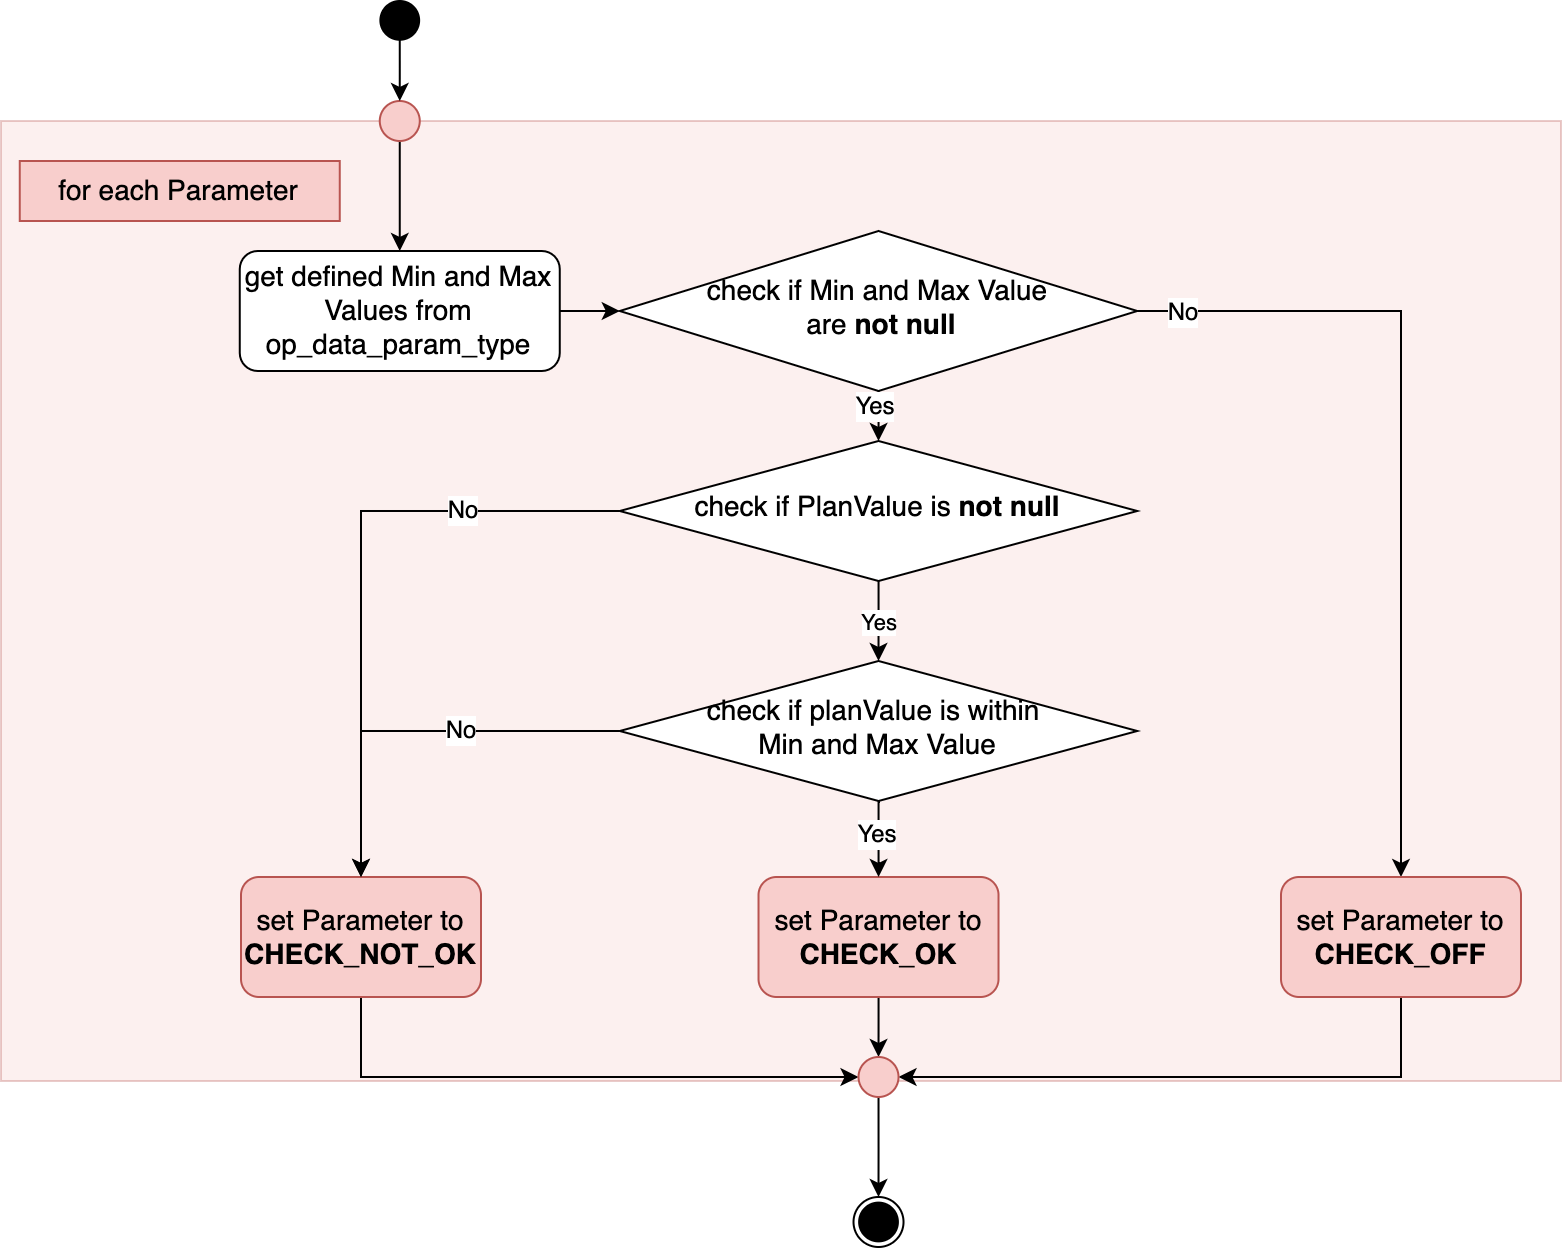
\includegraphics[width=0.80\paperwidth]{bilder/flowchart-condition-check-6-2.png}}
    \caption{Flussdiagramm des \gls{ConditionCheck}s}
    \label{fig:condition-check}
\end{figure}

\subsection{Equipment Check}

\begin{figure}[!htbp]
    \centering
    \makebox[\textwidth]{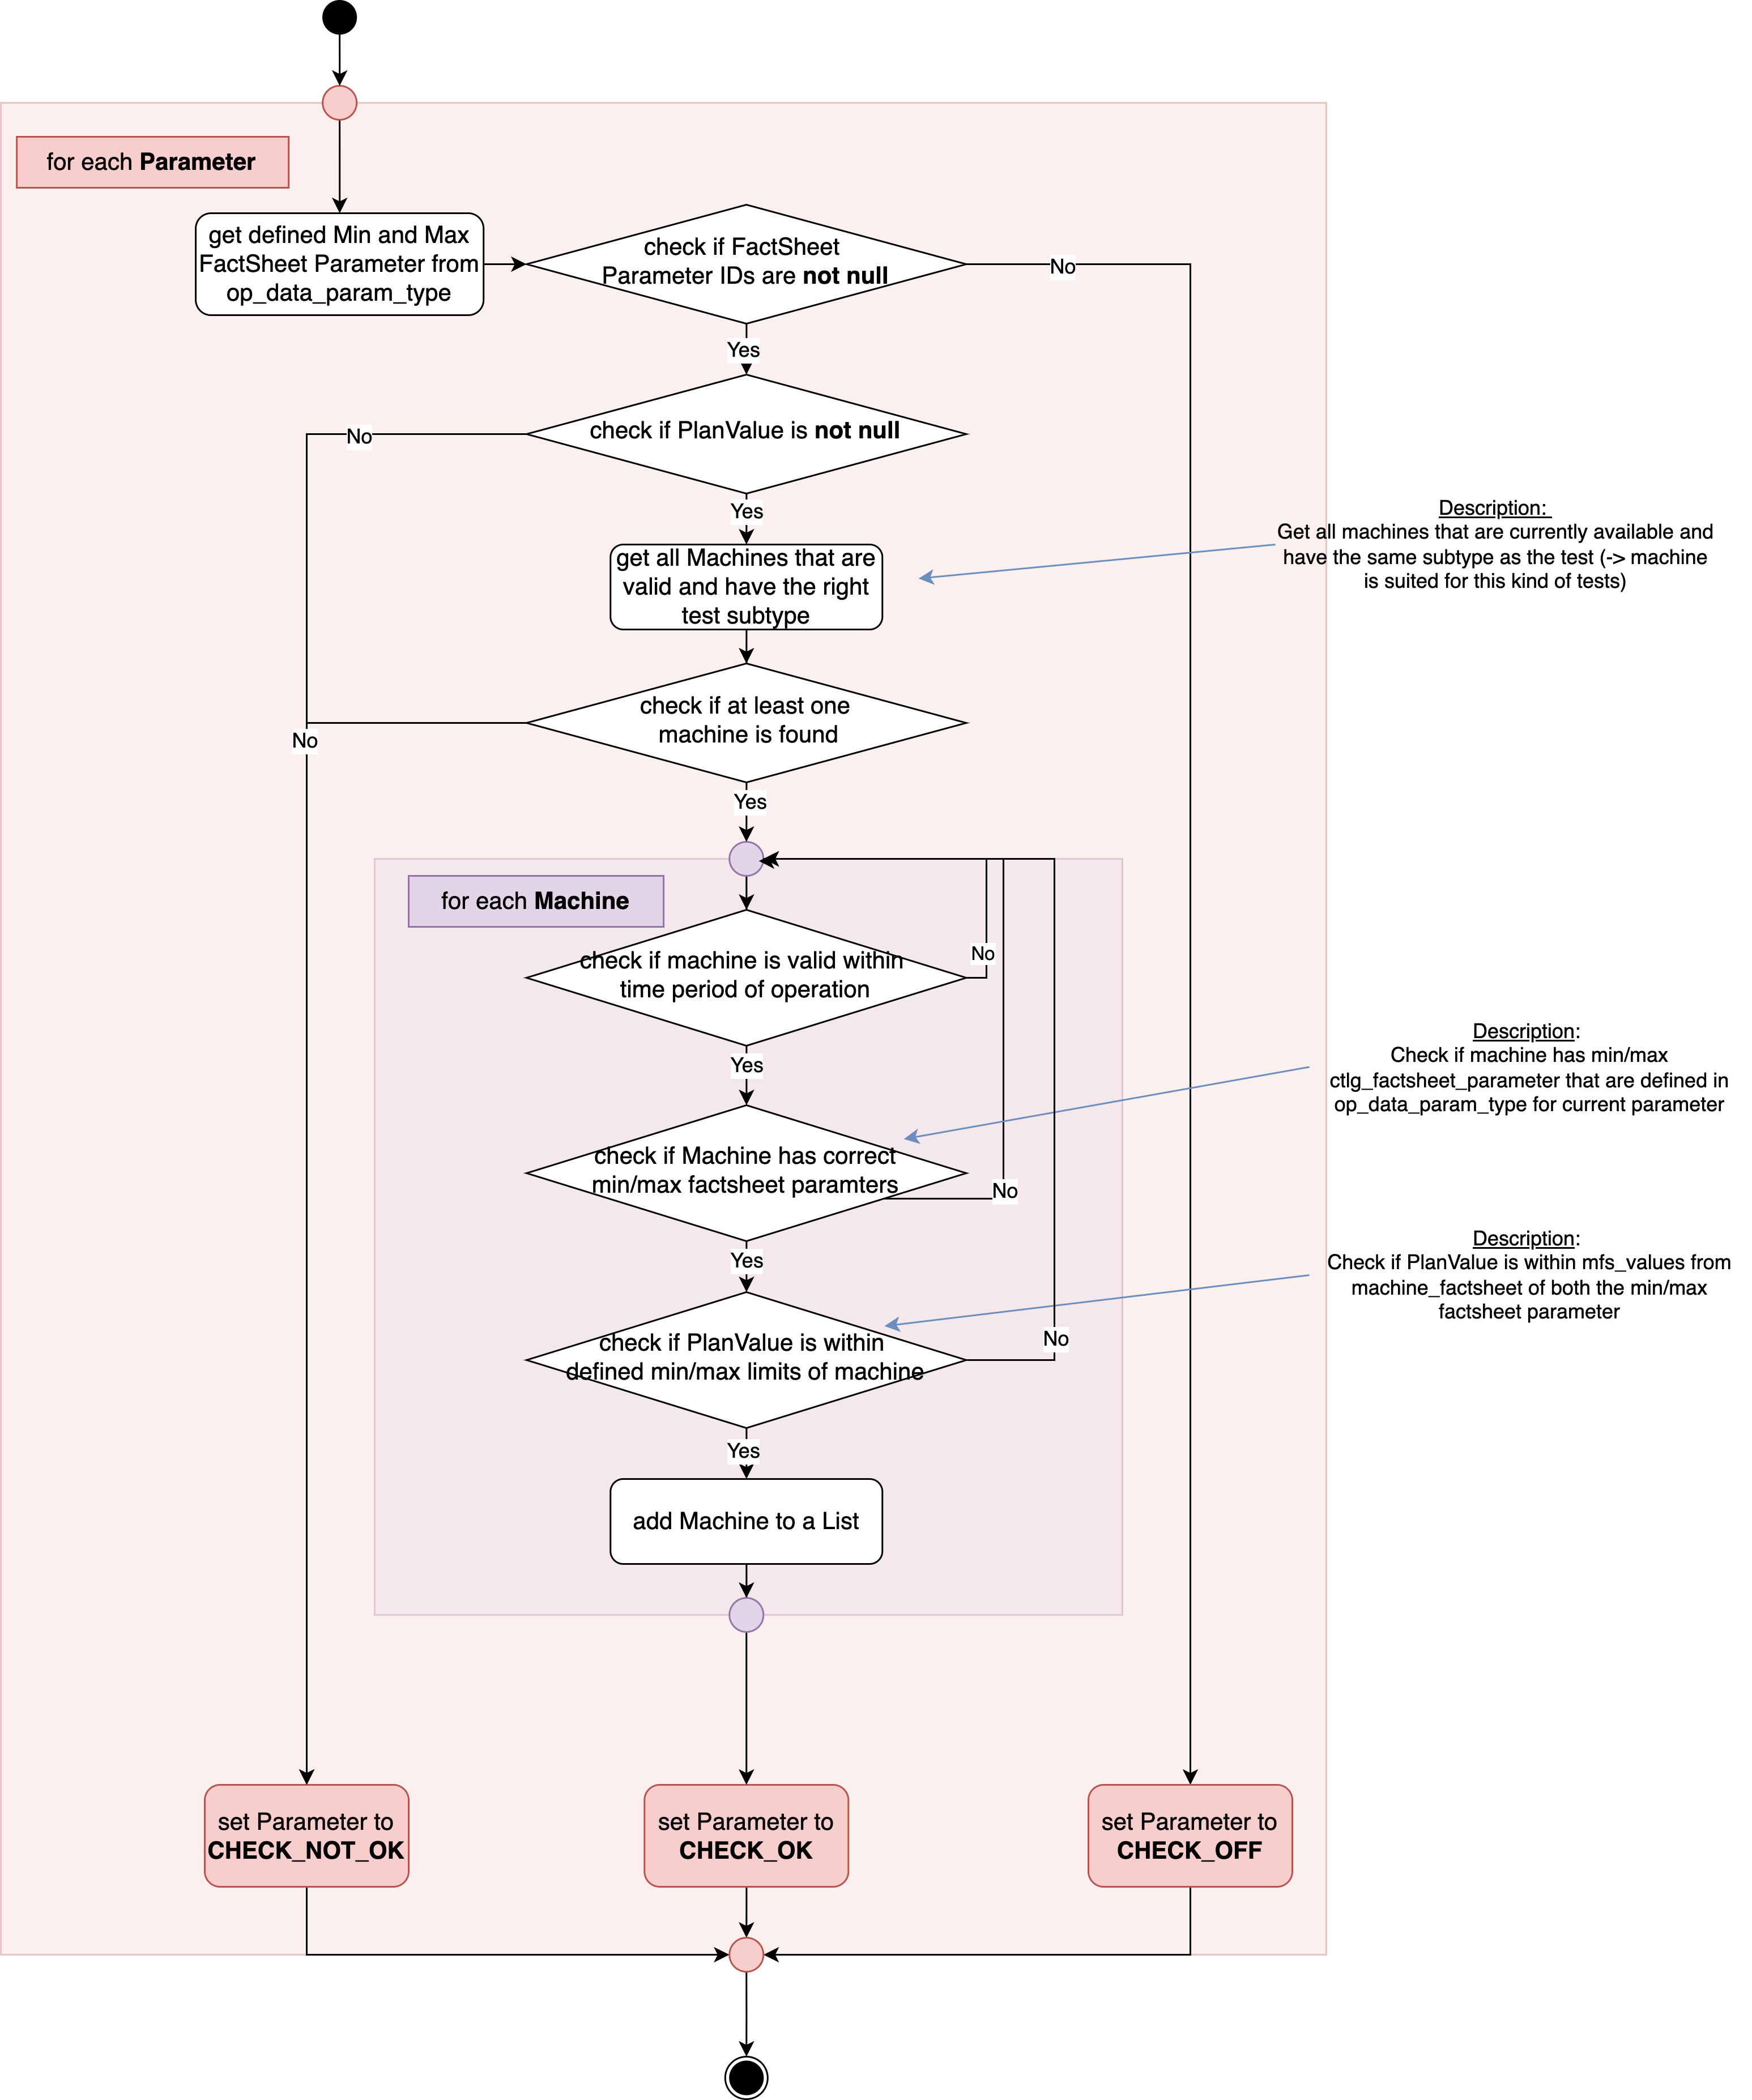
\includegraphics[width=0.85\paperwidth]{bilder/flowchart-equipment-check-6-2.png}}
    \caption{Flussdiagramm des \gls{EquipmentCheck}s}
    \label{fig:equipment-check}
\end{figure}

Der \gls{EquipmentCheck} ist in Abbildung \ref{fig:equipment-check} dargestellt. Der Prozess beginnt ebenfalls mit dem Abruf von Daten aus der passenden \texttt{op\_data\_param\_type} Tabelle. Falls keine Referenzen für den minimalen und maximalen Maschinenparameter (\texttt{ctlg\_factsheet\_parameter}) hinterlegt sind, ist die Überprüfung für diese Parameter, nicht erforderlich und ist somit beendet. Andernfalls muss sichergestellt werden, dass ein \textit{PlanValue} gesetzt ist. Erst danach startet der eigentliche Durchführbarkeits-Check.

Als erstes werden aus der Datenbank alle Maschinen abgerufen, die als ''valide'' gelten, also weder defekt noch in Wartung sind, und zudem den gleichen Testsubtypen aufweisen wie der zu prüfende Test. Die Zuordnung der Maschinen zu einem spezifischen Testsubtyp erfolgt dabei indirekt über die Verknüpfungstabelle \texttt{machine\_test\_sub\_type}, welche die Maschinen mit dem jeweiligen \texttt{ctlg\_test\_sub\_type} verknüpft.

Anschließend werden die verbleibenden Maschinen einzeln durchlaufen (siehe lila markierter Bereich in Abbildung \ref{fig:equipment-check}). Zuerst wird analysiert, ob die Maschine im geplanten Zeitraum der Operation zur Verfügung steht. Danach erfolgt die Überprüfung, ob die Maschine den Parameter grundsätzlich umsetzen kann. Dazu wird geprüft, ob die Maschine über die gleichen \texttt{ctlg\_factsheet\_parameter} verfügt, die in der Verknüpfungstabelle definiert sind. Falls dies der Fall ist, werden die minimalen und maximalen Werte über den zugehörigen Eintrag im Maschinen-Factsheet (\texttt{MFS\_VALUE}) abgerufen. Anschließend wird kontrolliert, ob der geplante Wert (\textit{PlanValue}) des Parameters innerhalb dieser Grenzen liegt. Ist dies der Fall, gilt die Maschine als geeignet, den geplanten Wert umzusetzen, und der Equipment-Check wird als erfolgreich betrachtet.

Alle Maschinen, die den Parameter mit dem geplanten Wert umsetzten können, werden in einer Liste als \texttt{check\_item\_result\_list} erfasst und mit dem zugehörigen \texttt{feasibility\_check\_item\_result} später in der Datenbank abgespeichert. 


\subsection{Benutzer Feedback}

Damit der Endnutzer das Ergebnis des Feasibility Checks nachvollziehen kann, wird jedem Feasibility-Resultat in der Datenbank eine spezifische, nutzerfreundliche Erklärung zugeordnet (\texttt{FCIR\_DESCRIPTION}). Diese Rückmeldungen sind nach den unterschiedlichen Überprüfungsebenen strukturiert, sodass der Benutzer präzise erkennen kann, an welcher Stelle Handlungsbedarf besteht. In folgenden Tabellen \ref{tab:feedback-test}, \ref{tab:feedback-operation}, \ref{tab:feedback-condition} und \ref{tab:feedback-equipment} werden die wichtigsten Rückmeldungen dargestellt.

Feasibility-Results mit dem Status \texttt{CHECK\_OFF} werden im Regelfall nicht gespeichert, da sie keine zusätzlichen, für den Benutzer relevanten Informationen liefern. Die Abspeicherung dieser Ergebnisse kann jedoch zu Debugging-Zwecken temporär aktiviert werden, um eine detailliertere Analyse der Prüfschritte zu ermöglichen.


\begin{table}[htb]
    \centering
    \footnotesize
    \renewcommand{\arraystretch}{1.1} % Erhöht den Zeilenabstand
    \setlength{\arrayrulewidth}{0.1pt} % Dünnere Linien
    \begin{tabular}{p{0.8\linewidth} p{0.15\linewidth}}
        \textbf{Meldung} & \textbf{Status} \\
        \midrule
        Feasibility Configuration not found & \texttt{CHECK\_OFF} \\
        \midrule
        Check Item is disabled for automatic feasibility check, see \texttt{ctlg\_feasibillity\_config} & \texttt{CHECK\_MANUAL} \\
        \midrule
        No Operations found for this test & \texttt{CHECK\_OFF} \\
        \bottomrule
    \end{tabular}
    \caption{Feedback auf Test-Ebene}
    \label{tab:feedback-test}
\end{table}


\begin{table}[htb]
    \centering
    \footnotesize
    \renewcommand{\arraystretch}{1.1}
    \begin{tabular}{p{0.8\linewidth} p{0.15\linewidth}}
        \textbf{Meldung} & \textbf{Status} \\
        \midrule
        Operation with no Parameters & \texttt{CHECK\_OFF} \\
        \bottomrule
    \end{tabular}
    \caption{Feedback auf Operations-Ebene}
    \label{tab:feedback-operation}
\end{table}


\begin{table}[htb]
    \centering
    \footnotesize
    \renewcommand{\arraystretch}{1.1}
    \begin{tabular}{p{0.8\linewidth} p{0.15\linewidth}}
        \textbf{Meldung} & \textbf{Status} \\
        \midrule
        No \texttt{op\_data\_param\_type} was found for this parameter & \texttt{CHECK\_NOT\_OK} \\
        \midrule
        No Conditions defined & \texttt{CHECK\_OFF} \\
        \midrule
        Error: PlanValue is not set & \texttt{CHECK\_NOT\_OK} \\
        \midrule
        Check successful: PlanValue=\{\textit{planValue}\}, ConditionMin=\{\textit{ConditionMin}\}, ConditionMax=\{\textit{ConditionMax}\} & \texttt{CHECK\_OK} \\
        \midrule
        Check failed: PlanValue=\{\textit{planValue}\}, ConditionMin=\{\textit{ConditionMin}\}, ConditionMax=\{\textit{ConditionMax}\} & \texttt{CHECK\_NOT\_OK} \\
        \bottomrule
    \end{tabular}
    \caption{Feedback auf Parameter-Ebene -- Condition Check}
    \label{tab:feedback-condition}
\end{table}


\begin{table}[htb]
    \centering
    \footnotesize
    \renewcommand{\arraystretch}{1.1}
    \begin{tabular}{p{0.8\linewidth} p{0.15\linewidth}}
        \textbf{Meldung} & \textbf{Status} \\
        \midrule
        No \texttt{op\_data\_param\_type} was found for this parameter & \texttt{CHECK\_NOT\_OK} \\
        \midrule
        No Equipment Parameters defined & \texttt{CHECK\_OFF} \\
        \midrule
        Error: PlanValue is not set & \texttt{CHECK\_NOT\_OK} \\
        \midrule
        Check failed: Found no valid machines with Testsubtype of Test & \texttt{CHECK\_NOT\_OK} \\
        \midrule
        Check successful: Found \{\textit{numberOfMachines}\} Machines for: PlanValue=\{\textit{planValue}\}, EquipmentParameterMin=\{\textit{ParameterMin}\}, EquipmentParameterMax=\{\textit{ParameterMax}\} & \texttt{CHECK\_OK} \\
        \midrule
        Check failed: Found no Machines: ... & \texttt{CHECK\_NOT\_OK} \\
        \quad Reason: Found no valid Machine within time period ... & \\
        \quad Reason: Found no valid Machine with needed Parameters ... & \\
        \quad Reason: Current PlanValue=\{\textit{planValue}\} too high: Please set PlanValue lower & \\
        \quad Reason: Current PlanValue=\{\textit{planValue}\} too low: Please set PlanValue higher & \\
        \bottomrule
    \end{tabular}
    \caption{Feedback auf Parameter-Ebene -- Equipment Check}
    \label{tab:feedback-equipment}
\end{table}



Die dargestellten Rückmeldungen ermöglichen es dem Benutzer, gezielt auf erkannte Probleme zu reagieren. So kann er beispielsweise den PlanValue anpassen, wenn in Tabelle~\ref{tab:feedback-equipment} darauf hingewiesen wird, dass der aktuelle Wert zu hoch oder zu niedrig ist. Diese detaillierte Information unterstützt den Benutzer bei der Identifikation und Behebung von Konfigurationsproblemen.


